\documentclass[]{article}
\usepackage{lmodern}
\usepackage{amssymb,amsmath}
\usepackage{ifxetex,ifluatex}
\usepackage{fixltx2e} % provides \textsubscript
\ifnum 0\ifxetex 1\fi\ifluatex 1\fi=0 % if pdftex
  \usepackage[T1]{fontenc}
  \usepackage[utf8]{inputenc}
\else % if luatex or xelatex
  \ifxetex
    \usepackage{mathspec}
    \usepackage{xltxtra,xunicode}
  \else
    \usepackage{fontspec}
  \fi
  \defaultfontfeatures{Mapping=tex-text,Scale=MatchLowercase}
  \newcommand{\euro}{€}
\fi
% use upquote if available, for straight quotes in verbatim environments
\IfFileExists{upquote.sty}{\usepackage{upquote}}{}
% use microtype if available
\IfFileExists{microtype.sty}{%
\usepackage{microtype}
\UseMicrotypeSet[protrusion]{basicmath} % disable protrusion for tt fonts
}{}
\usepackage[margin=1in]{geometry}
\usepackage{graphicx}
\makeatletter
\def\maxwidth{\ifdim\Gin@nat@width>\linewidth\linewidth\else\Gin@nat@width\fi}
\def\maxheight{\ifdim\Gin@nat@height>\textheight\textheight\else\Gin@nat@height\fi}
\makeatother
% Scale images if necessary, so that they will not overflow the page
% margins by default, and it is still possible to overwrite the defaults
% using explicit options in \includegraphics[width, height, ...]{}
\setkeys{Gin}{width=\maxwidth,height=\maxheight,keepaspectratio}
\ifxetex
  \usepackage[setpagesize=false, % page size defined by xetex
              unicode=false, % unicode breaks when used with xetex
              xetex]{hyperref}
\else
  \usepackage[unicode=true]{hyperref}
\fi
\hypersetup{breaklinks=true,
            bookmarks=true,
            pdfauthor={jcb},
            pdftitle={Completude},
            colorlinks=true,
            citecolor=blue,
            urlcolor=blue,
            linkcolor=magenta,
            pdfborder={0 0 0}}
\urlstyle{same}  % don't use monospace font for urls
\setlength{\parindent}{0pt}
\setlength{\parskip}{6pt plus 2pt minus 1pt}
\setlength{\emergencystretch}{3em}  % prevent overfull lines
\setcounter{secnumdepth}{5}

%%% Use protect on footnotes to avoid problems with footnotes in titles
\let\rmarkdownfootnote\footnote%
\def\footnote{\protect\rmarkdownfootnote}

%%% Change title format to be more compact
\usepackage{titling}

% Create subtitle command for use in maketitle
\newcommand{\subtitle}[1]{
  \posttitle{
    \begin{center}\large#1\end{center}
    }
}

\setlength{\droptitle}{-2em}
  \title{Completude}
  \pretitle{\vspace{\droptitle}\centering\huge}
  \posttitle{\par}
  \author{jcb}
  \preauthor{\centering\large\emph}
  \postauthor{\par}
  \predate{\centering\large\emph}
  \postdate{\par}
  \date{30 mars 2015}



\begin{document}

\maketitle


{
\hypersetup{linkcolor=black}
\setcounter{tocdepth}{2}
\tableofcontents
}
\section{Complétude des données}\label{completude-des-donnees}

Score de completude = somme des complétudes de chaque item.

Ce chapitre utilise le fichier
source(``../../RESURAL/Trame\_commune/rapport\_2014.R'') qui possède
deux fonctions pour calculer la complétude et dessiner le diagramme en
radar correspondant.

\subsection{Complétude régionale}\label{completude-regionale}

C'est la complétude calculée pour tous les RPU quelque soit
l'établissement producteur.

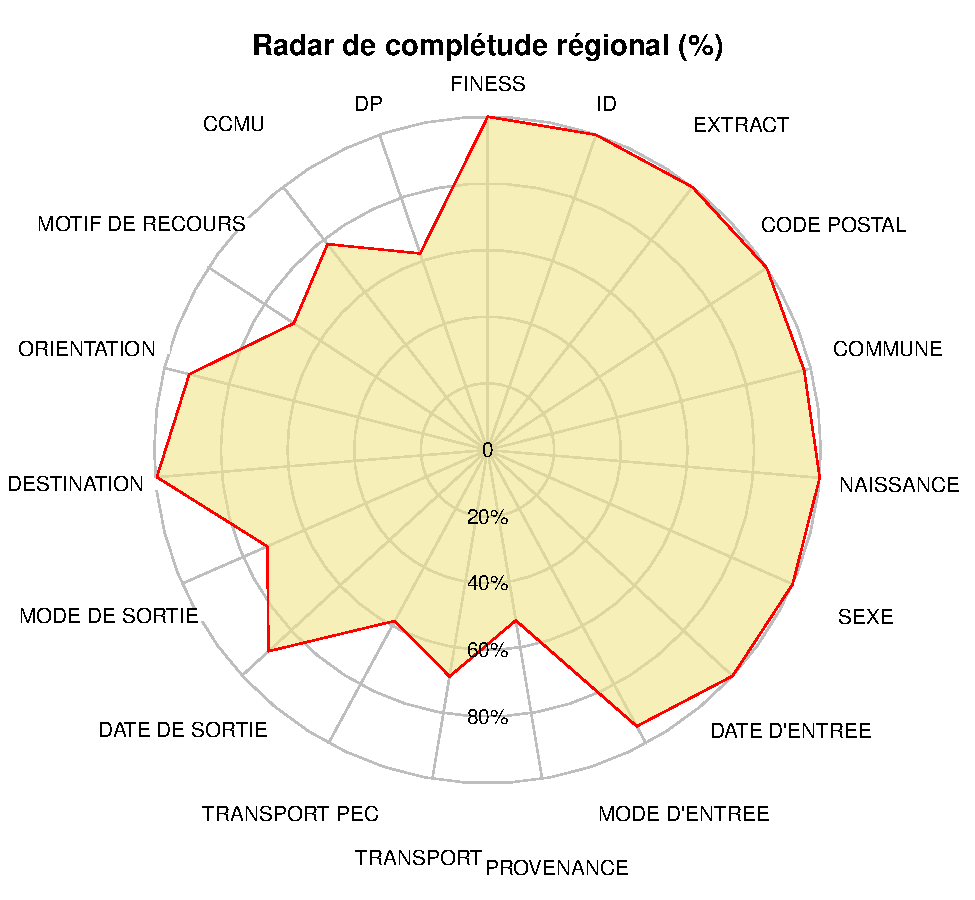
\includegraphics{completude_files/figure-latex/comp_regionale-1.pdf}

Score de complétude régional: 85.67 sur 100.

\subsection{Completude par
établissement}\label{completude-par-etablissement}

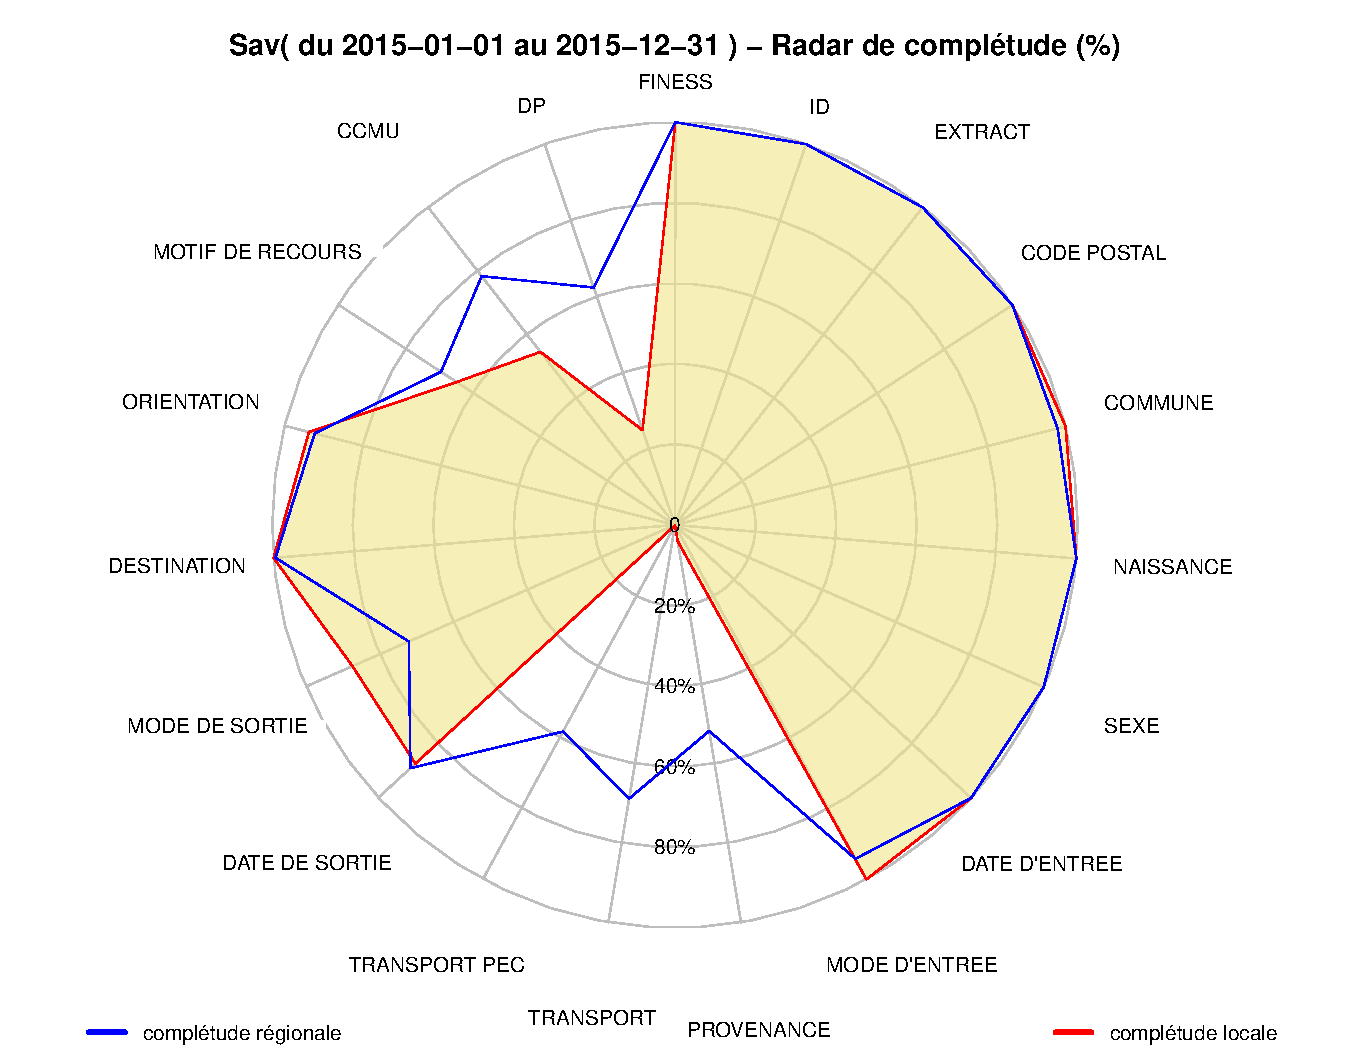
\includegraphics{completude_files/figure-latex/finess-1.pdf}

\begin{verbatim}
## Score local: 73.01  sur 100
\end{verbatim}

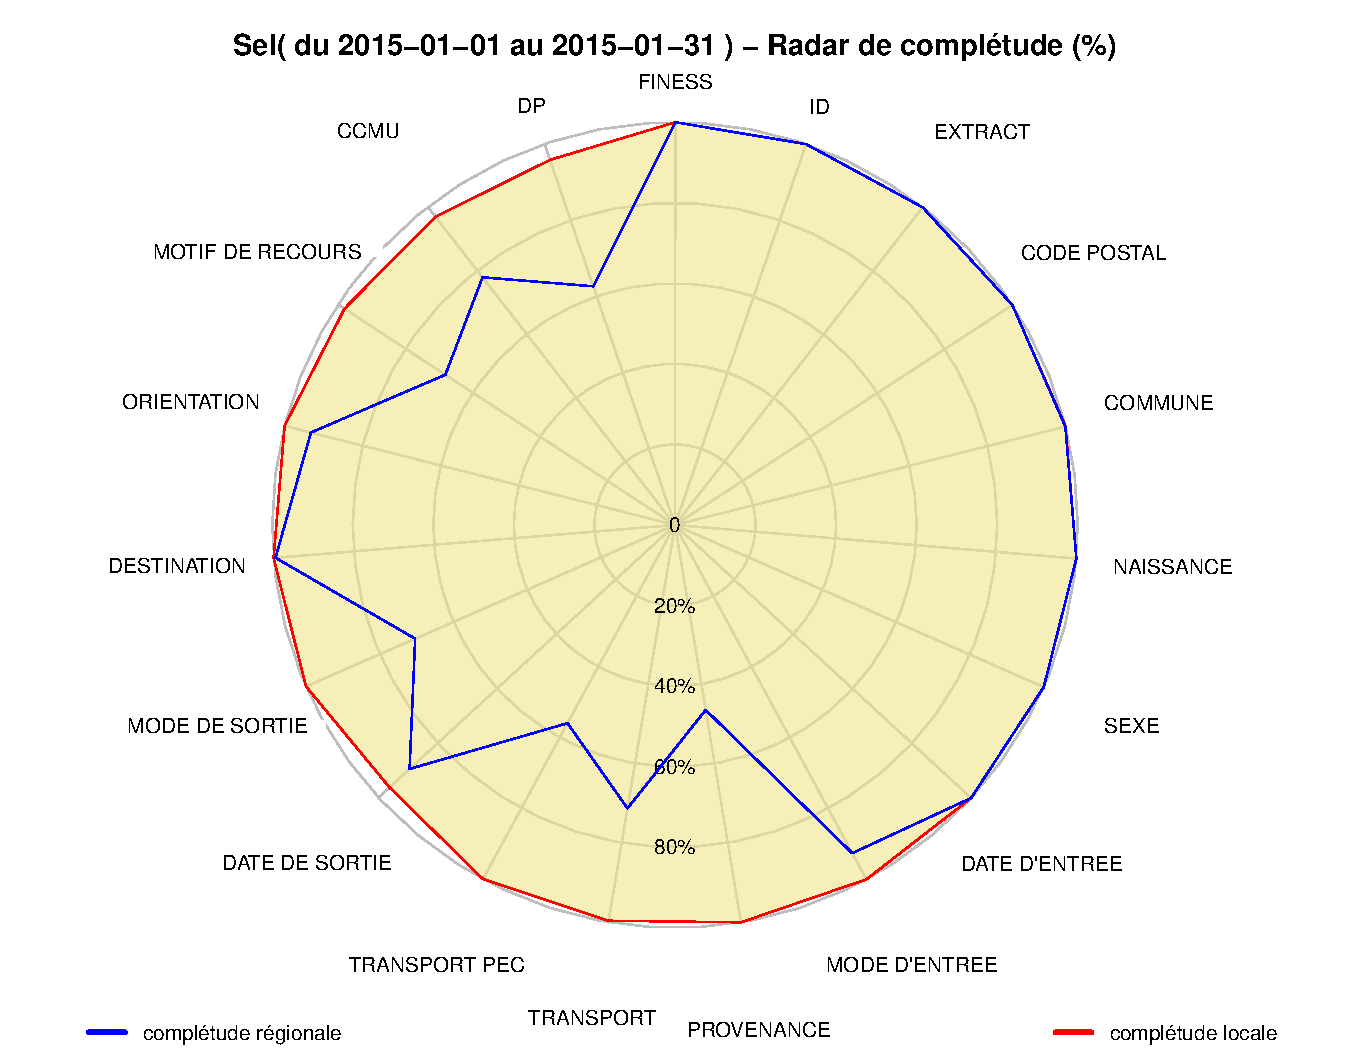
\includegraphics{completude_files/figure-latex/finess-2.pdf}

\begin{verbatim}
## Score local: 99.3  sur 100
\end{verbatim}

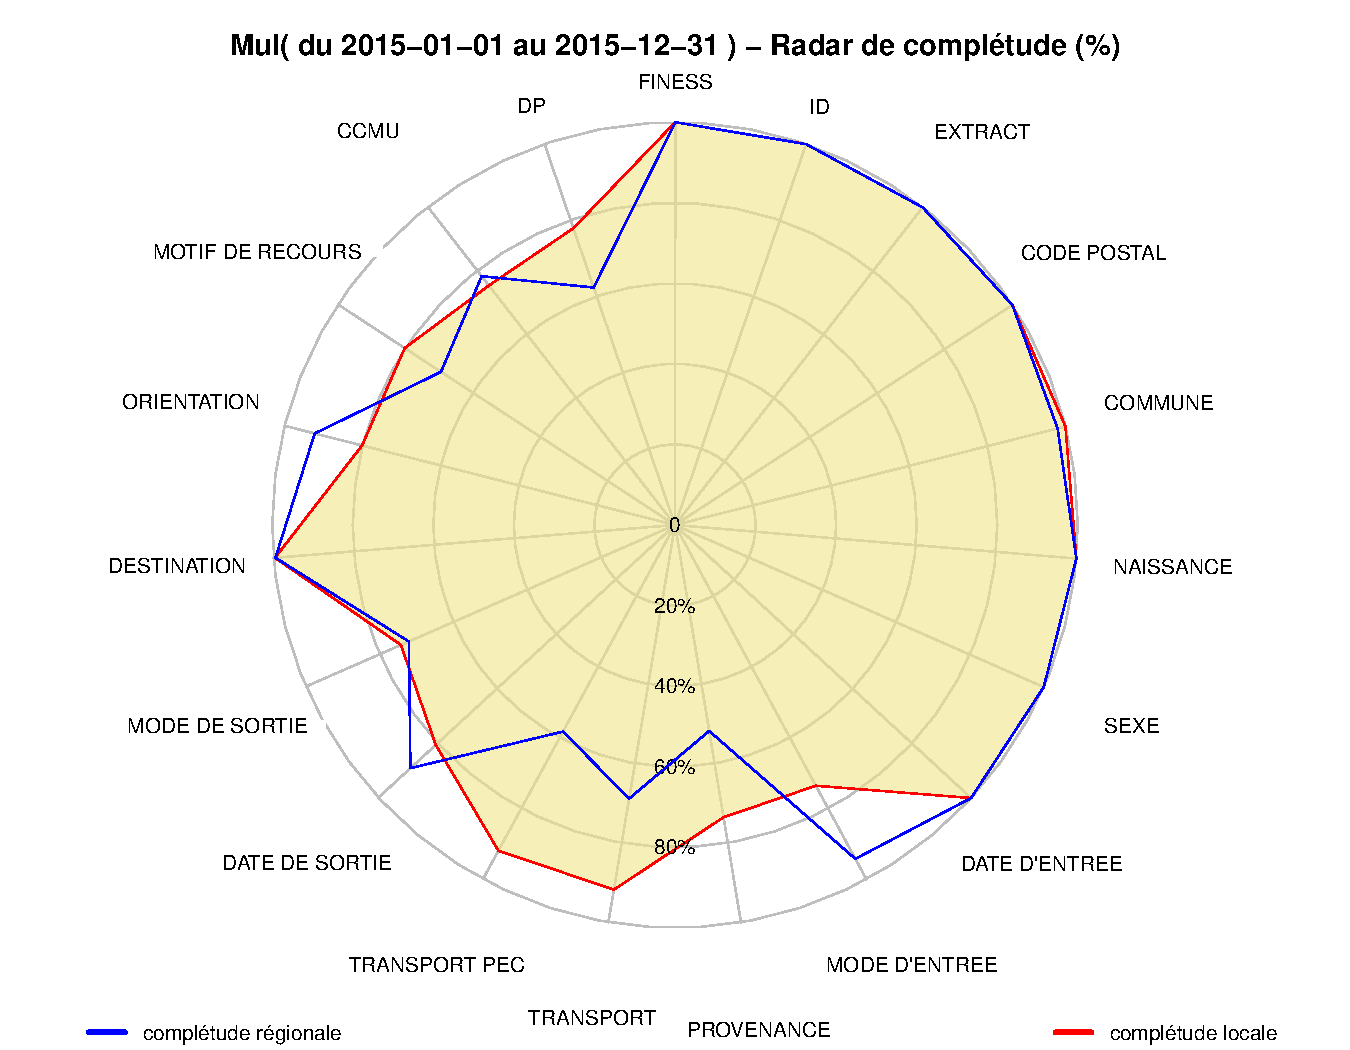
\includegraphics{completude_files/figure-latex/finess-3.pdf}

\begin{verbatim}
## Score local: 89.39  sur 100
\end{verbatim}

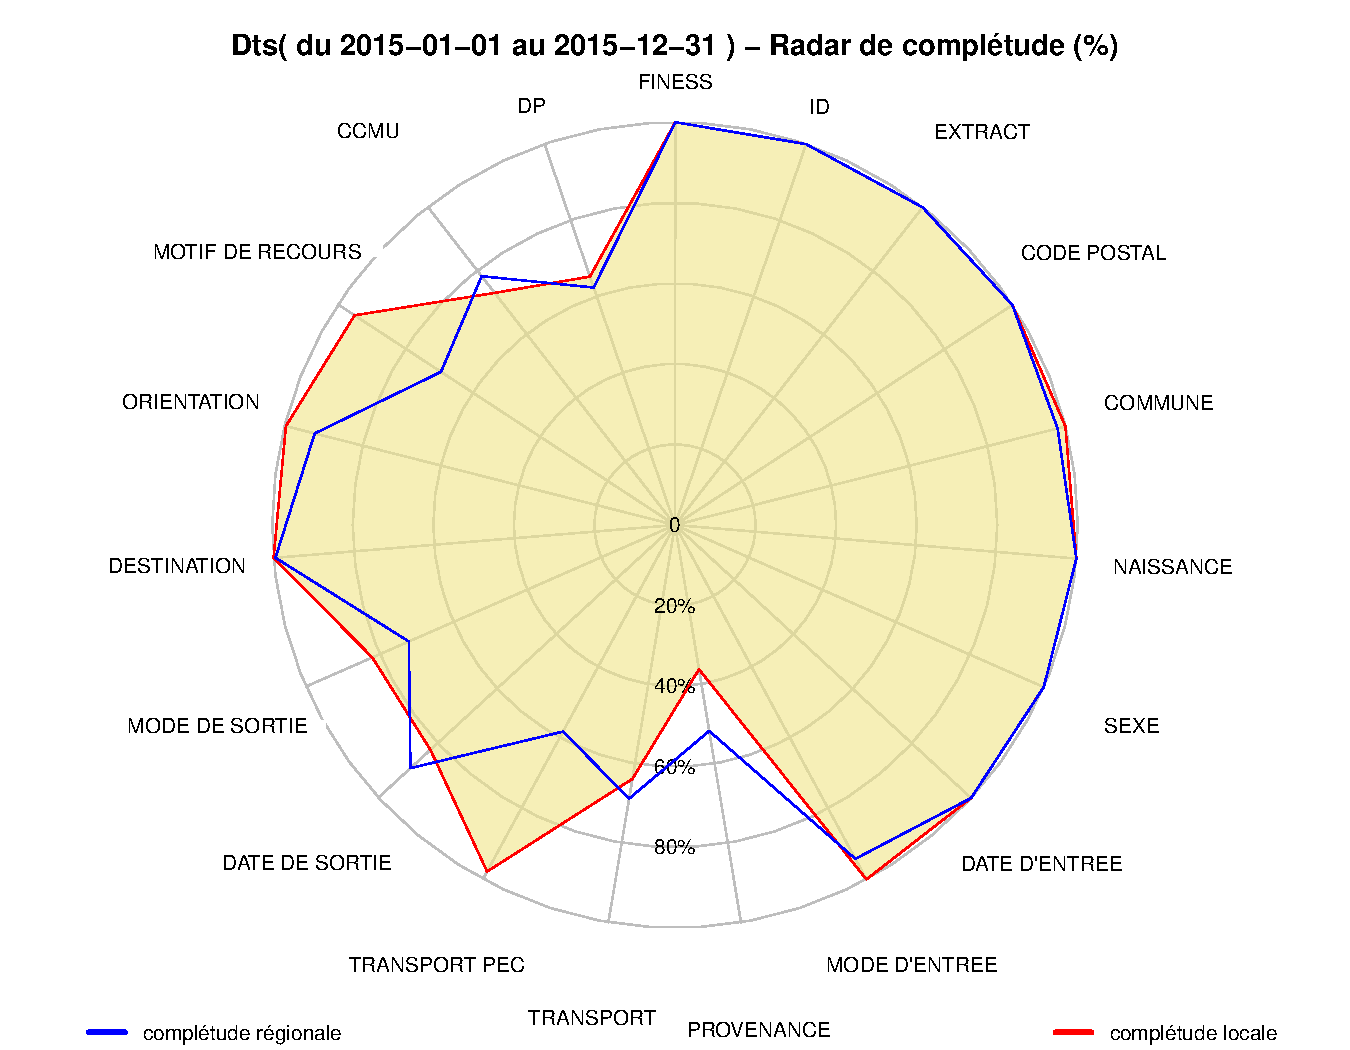
\includegraphics{completude_files/figure-latex/finess-4.pdf}

\begin{verbatim}
## Score local: 92.36  sur 100
\end{verbatim}

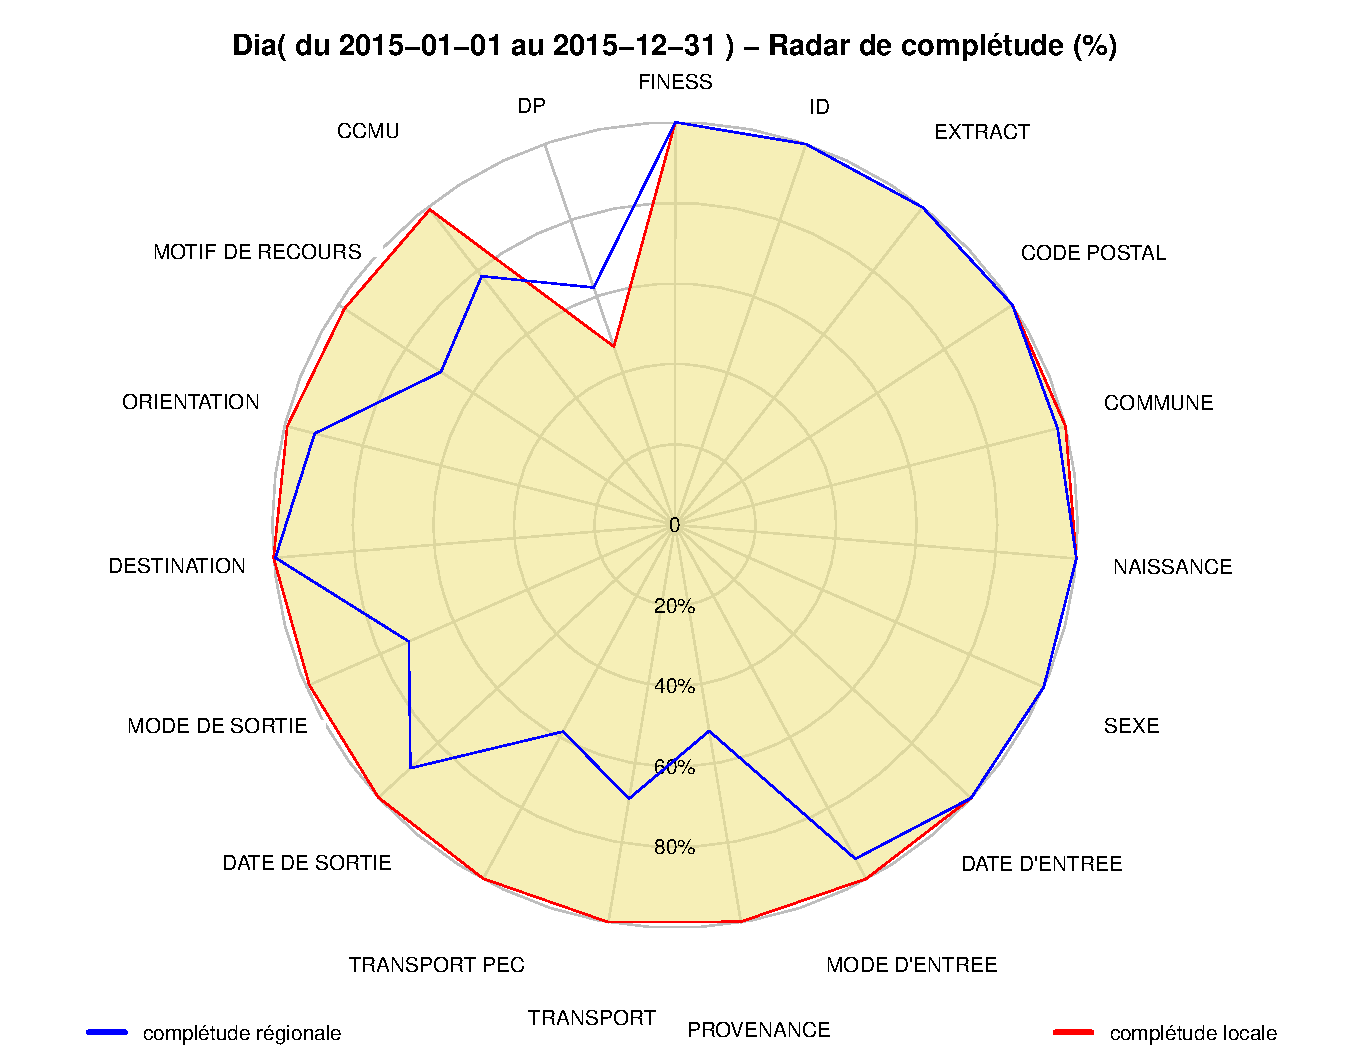
\includegraphics{completude_files/figure-latex/finess-5.pdf}

\begin{verbatim}
## Score local: 96  sur 100
\end{verbatim}

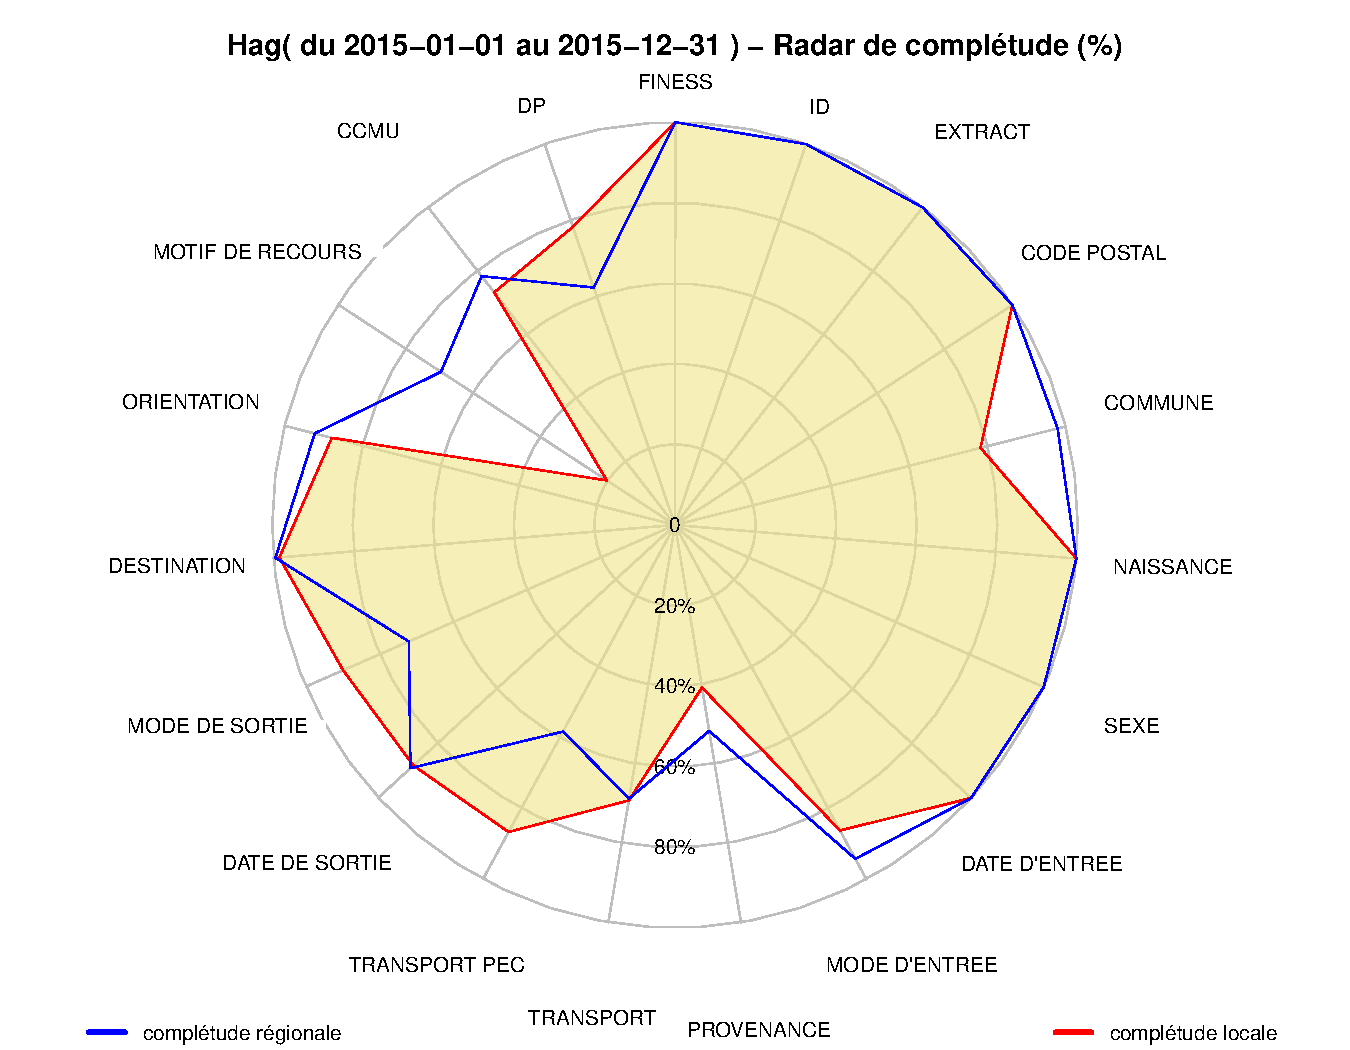
\includegraphics{completude_files/figure-latex/finess-6.pdf}

\begin{verbatim}
## Score local: 84.48  sur 100
\end{verbatim}

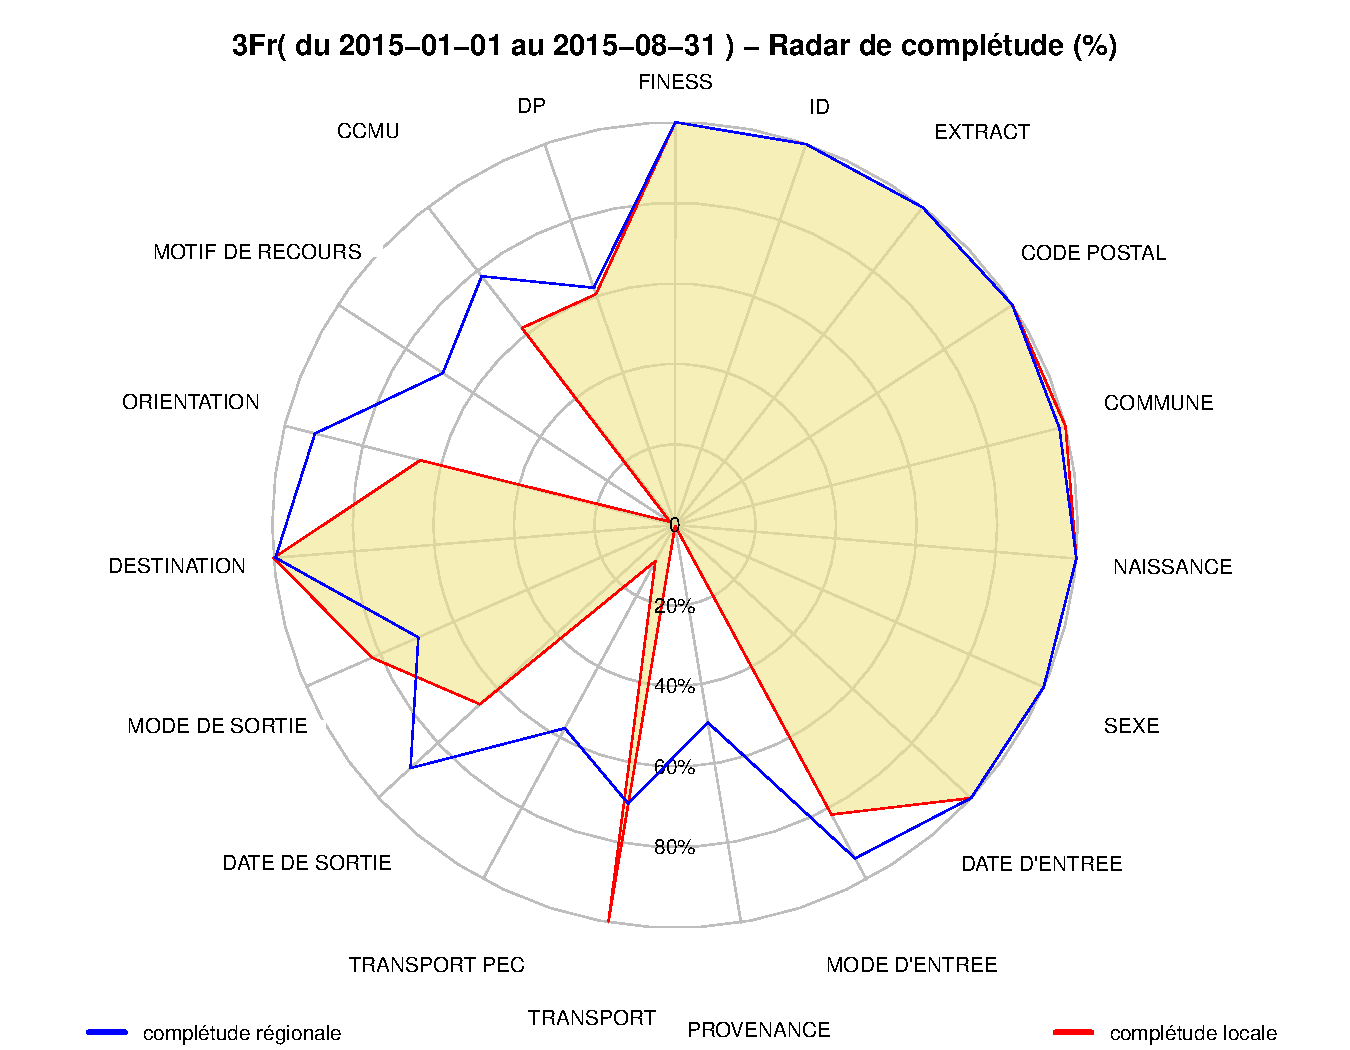
\includegraphics{completude_files/figure-latex/finess-7.pdf}

\begin{verbatim}
## Score local: 72.19  sur 100
\end{verbatim}

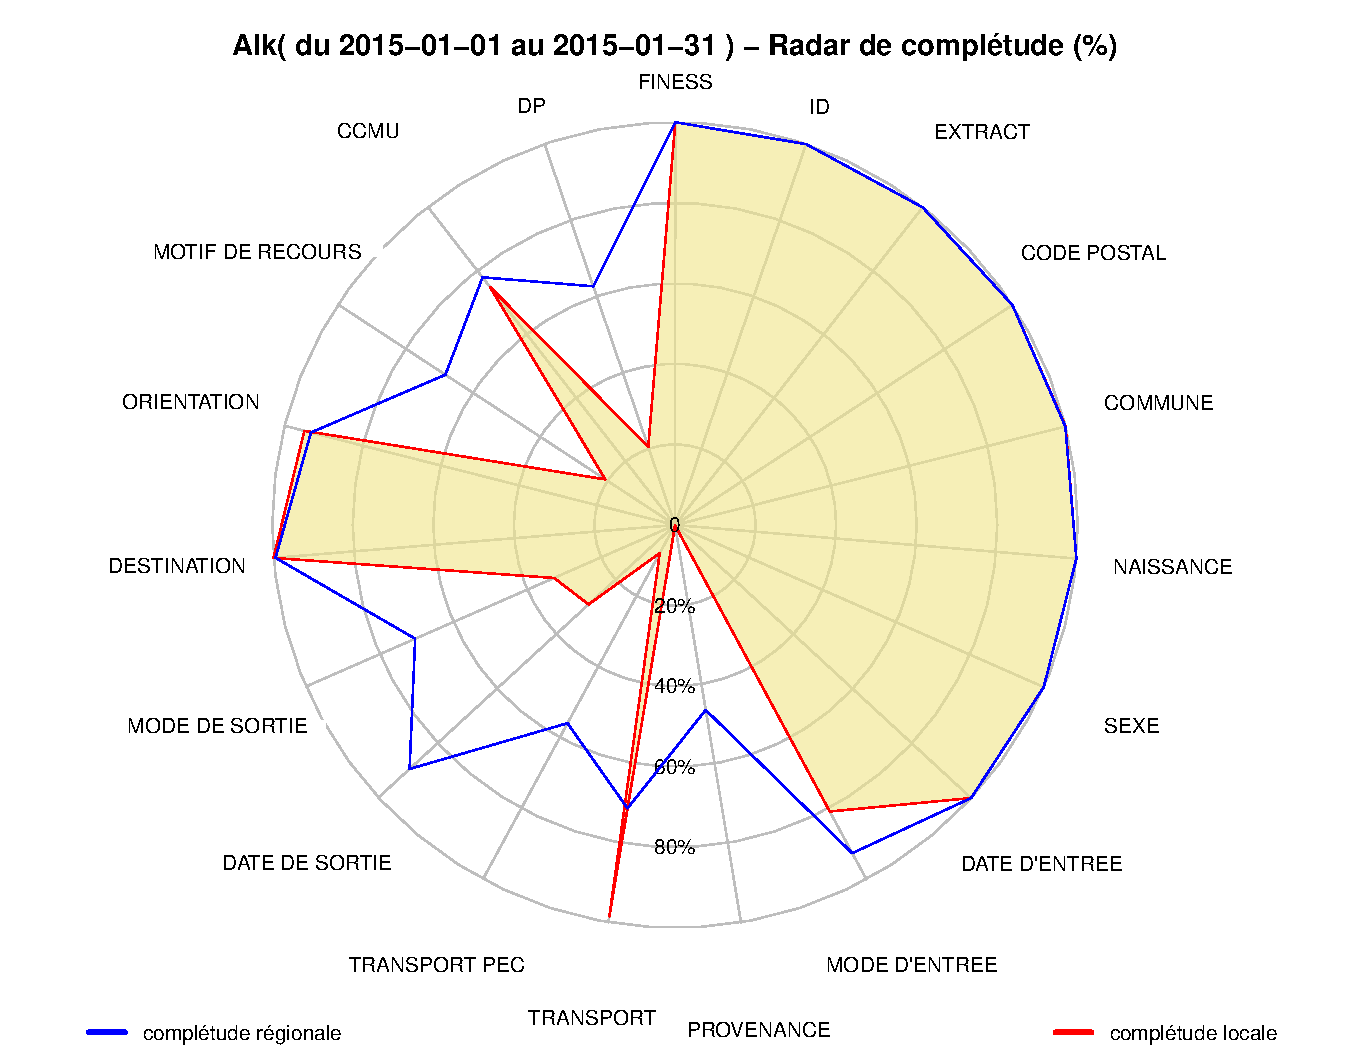
\includegraphics{completude_files/figure-latex/finess-8.pdf}

\begin{verbatim}
## Score local: 71.59  sur 100
\end{verbatim}

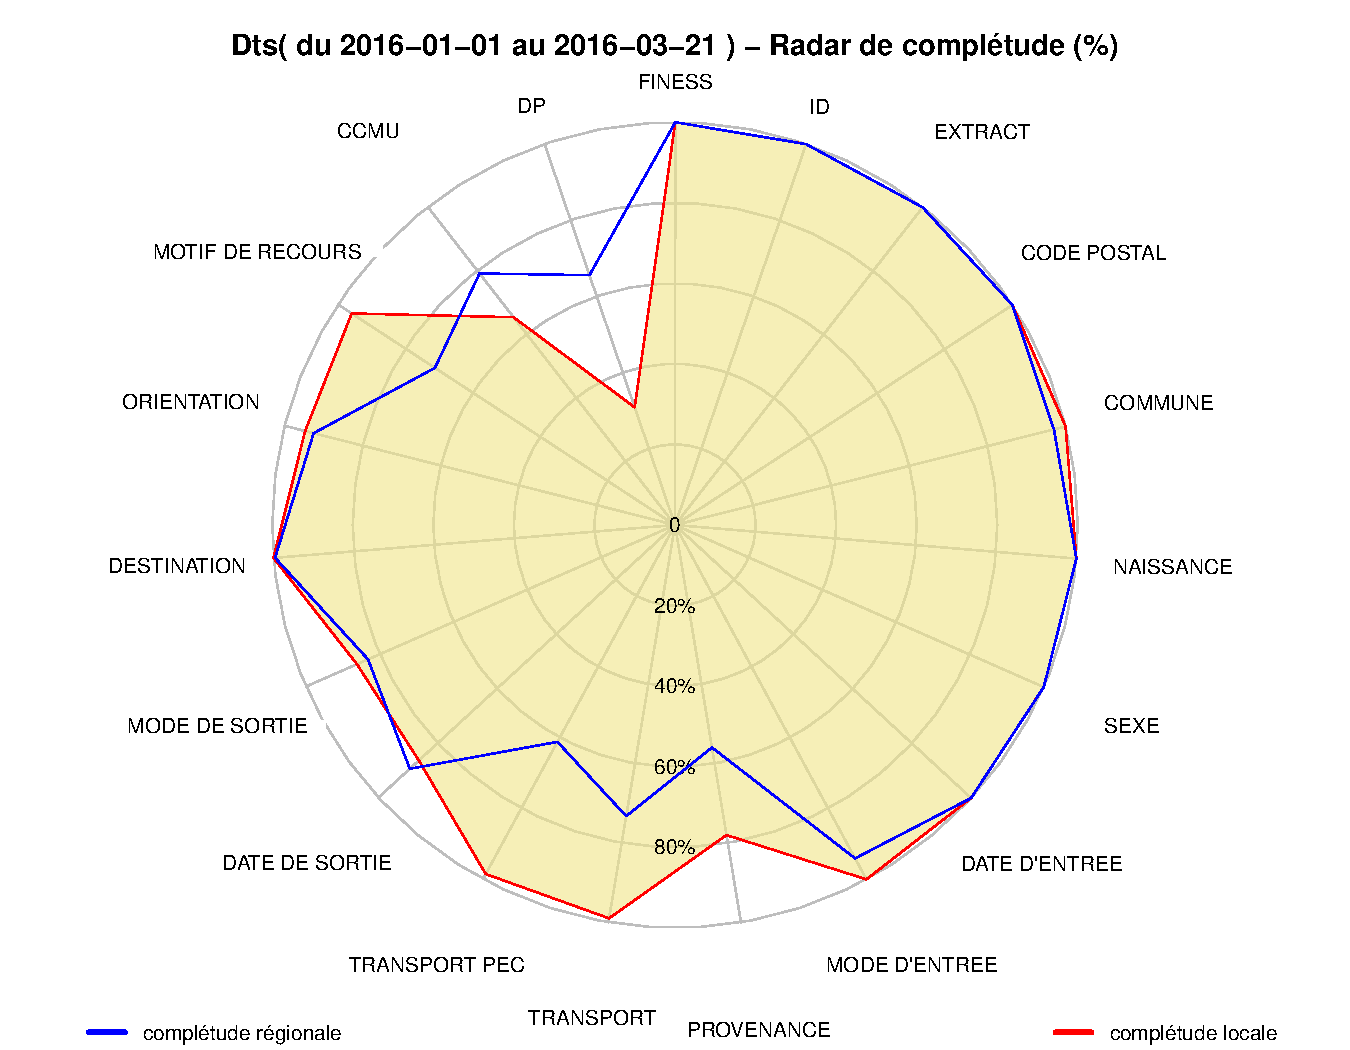
\includegraphics{completude_files/figure-latex/finess-9.pdf}

\begin{verbatim}
## Score local: 74.82  sur 100
\end{verbatim}

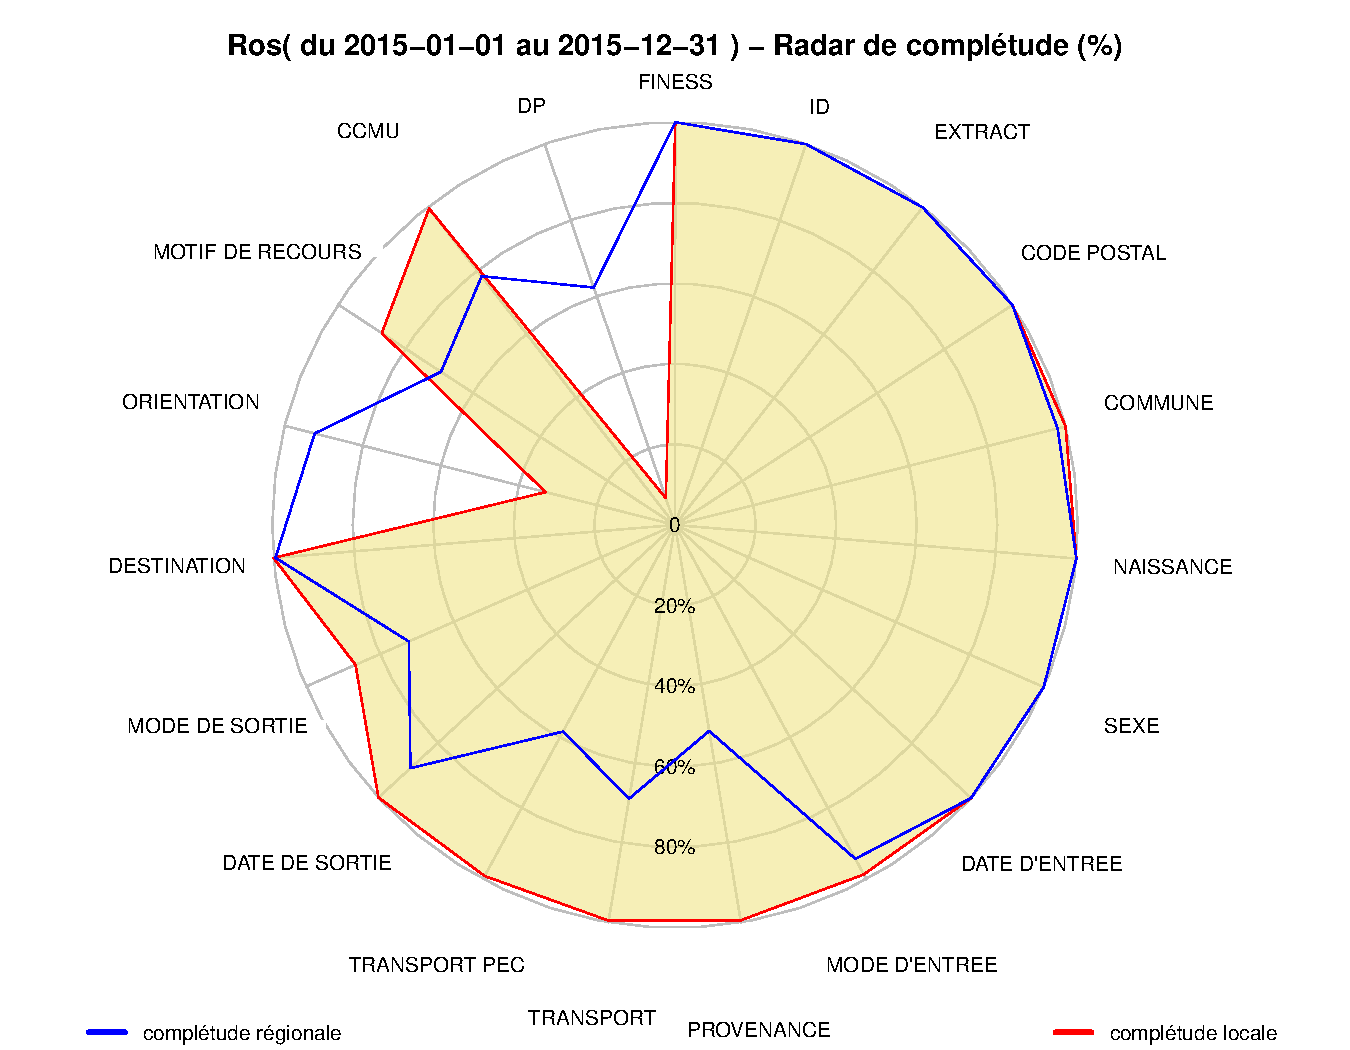
\includegraphics{completude_files/figure-latex/finess-10.pdf}

\begin{verbatim}
## Score local: 98.41  sur 100
\end{verbatim}

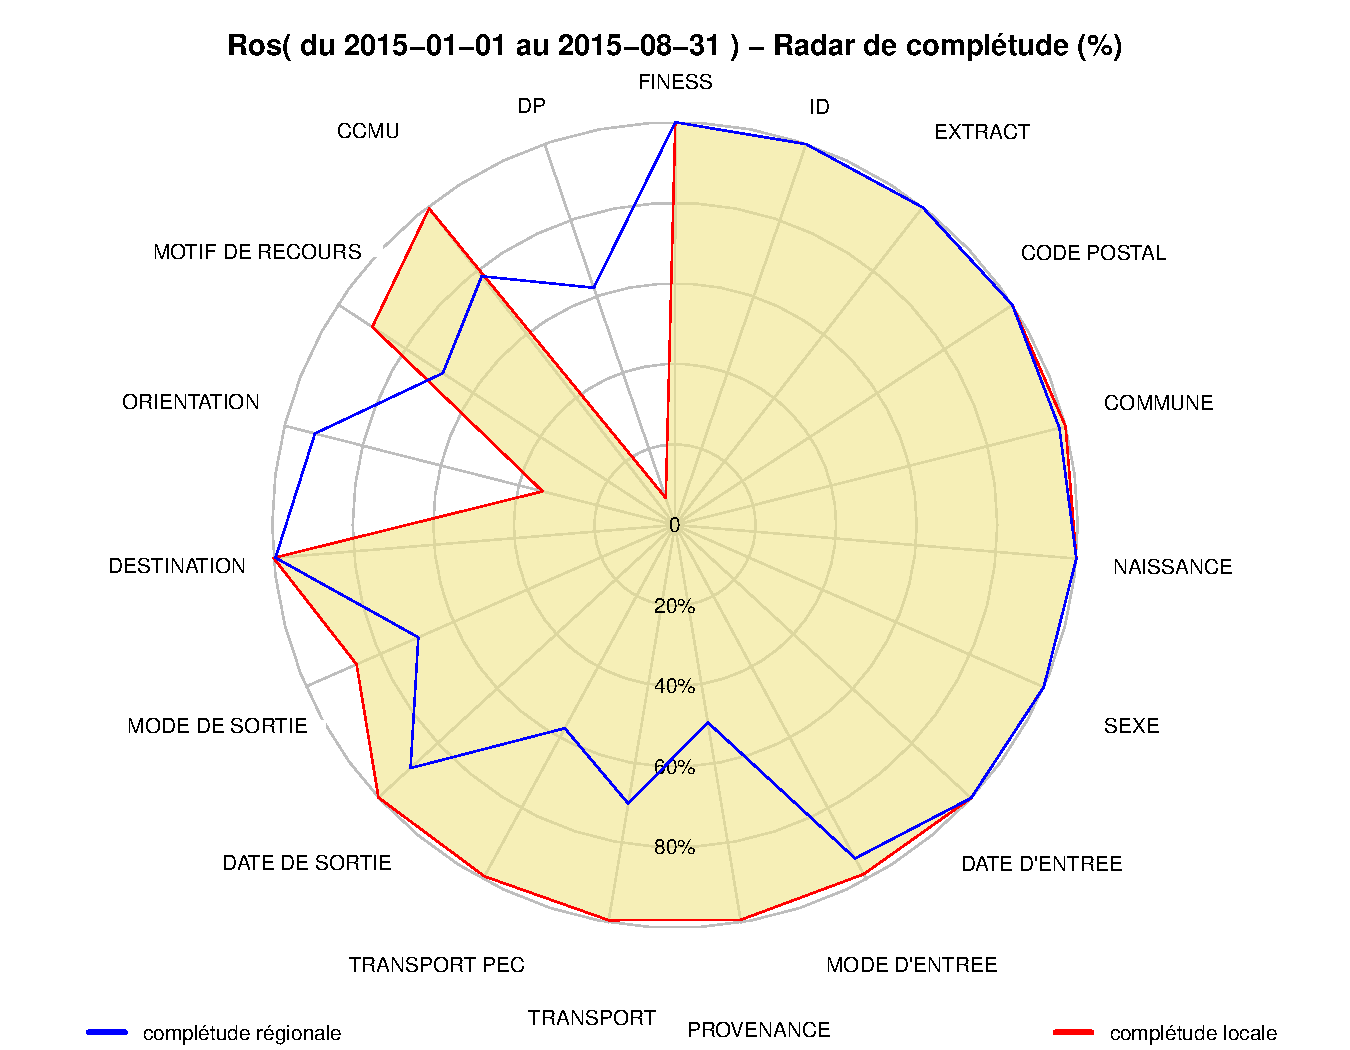
\includegraphics{completude_files/figure-latex/finess-11.pdf}

\begin{verbatim}
## Score local: 90.39  sur 100
\end{verbatim}

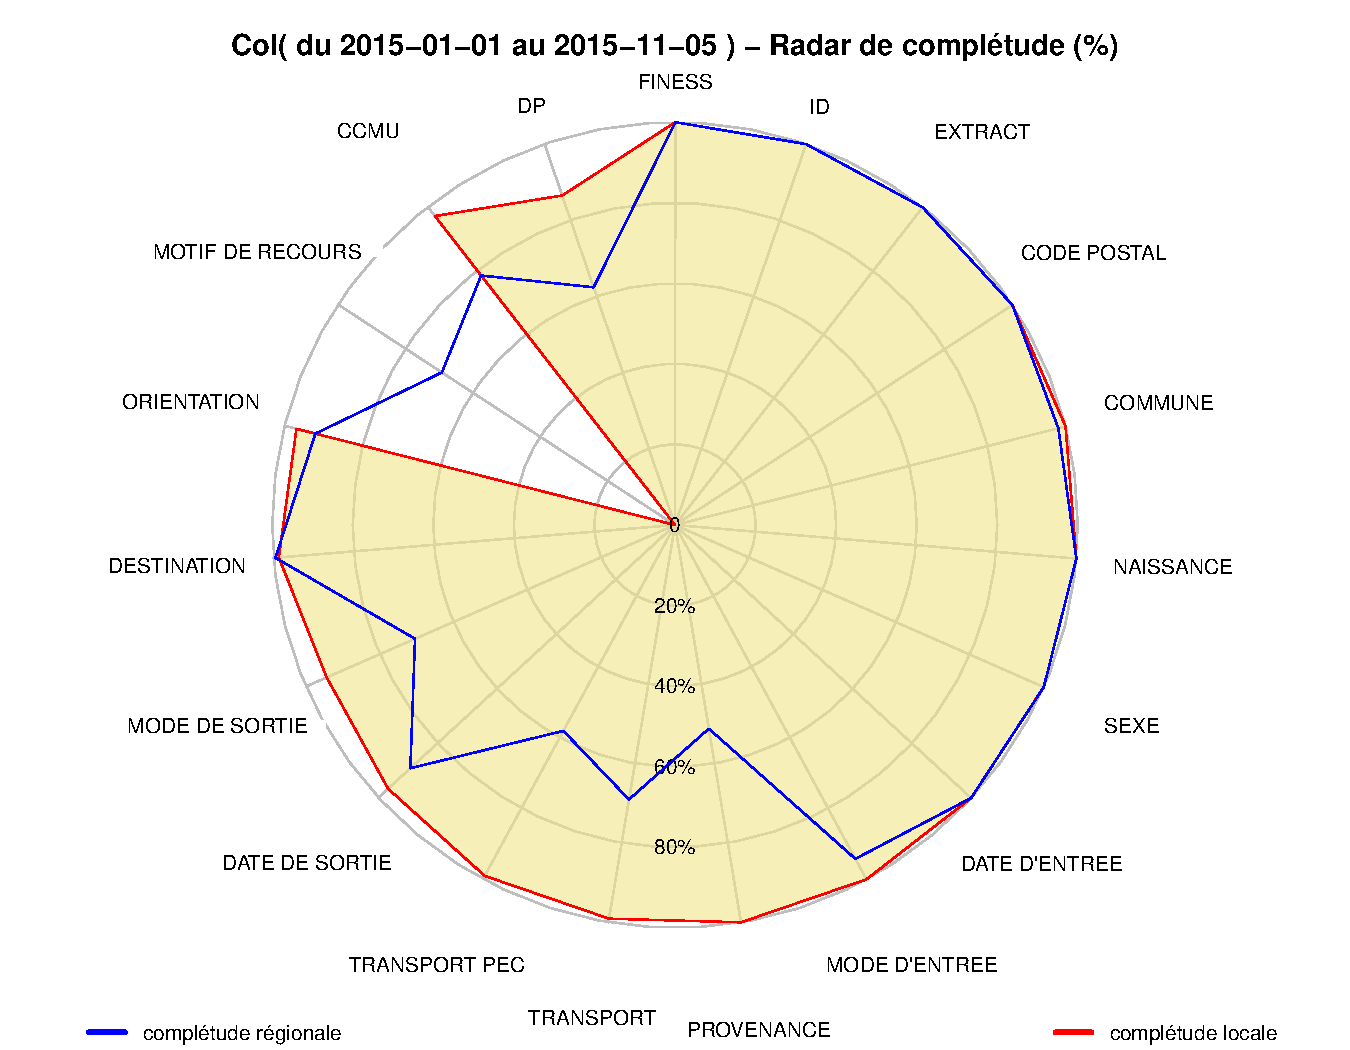
\includegraphics{completude_files/figure-latex/finess-12.pdf}

\begin{verbatim}
## Score local: 91.58  sur 100
\end{verbatim}

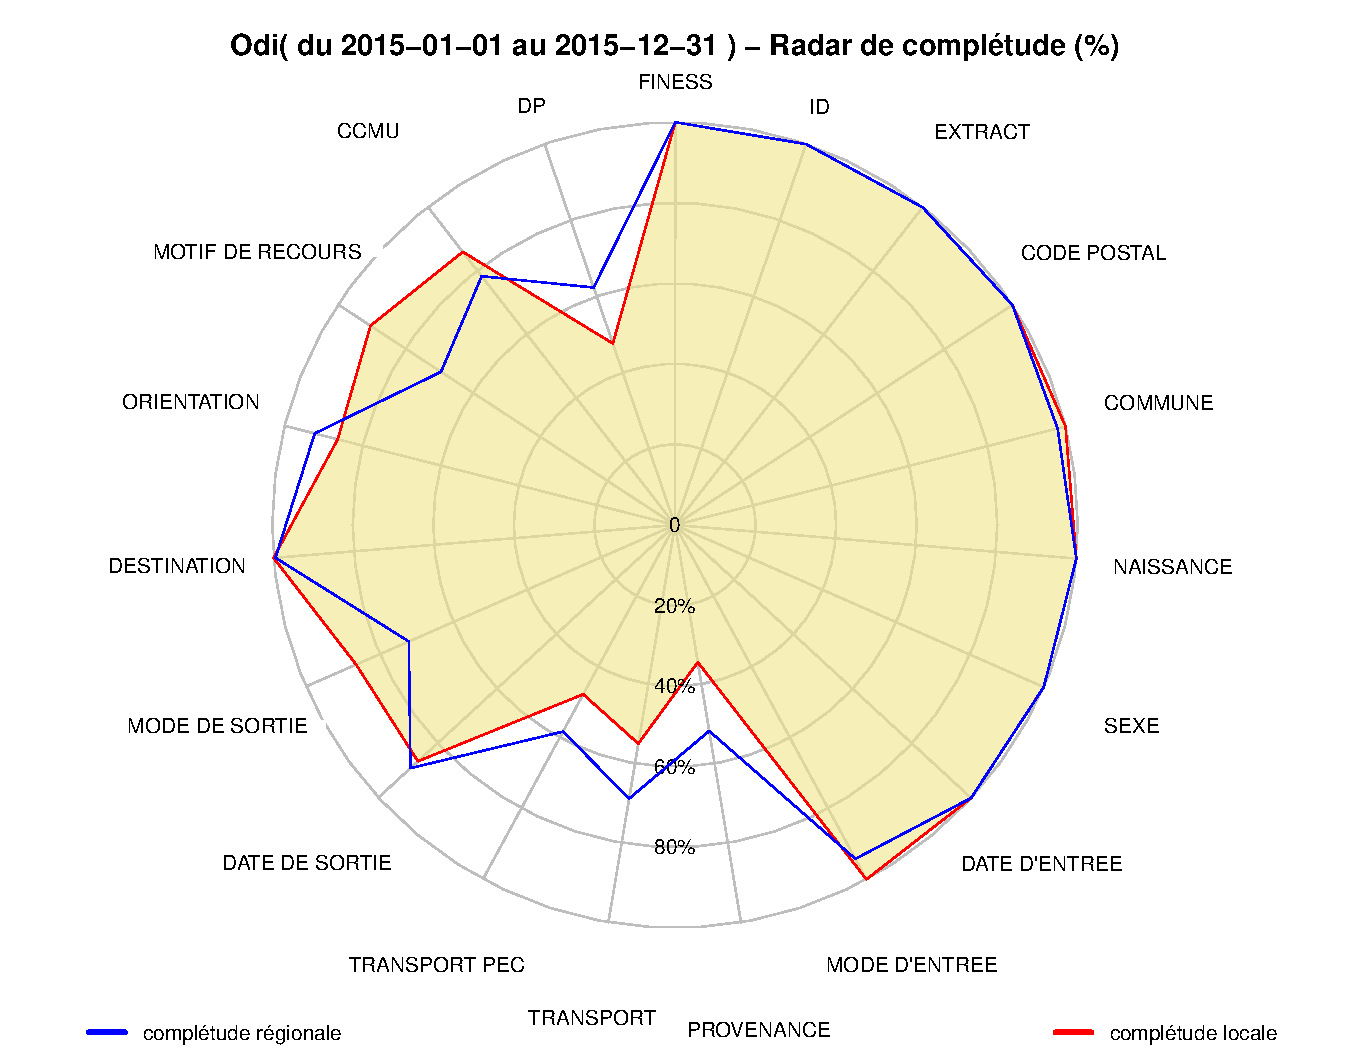
\includegraphics{completude_files/figure-latex/finess-13.pdf}

\begin{verbatim}
## Score local: 98.79  sur 100
\end{verbatim}

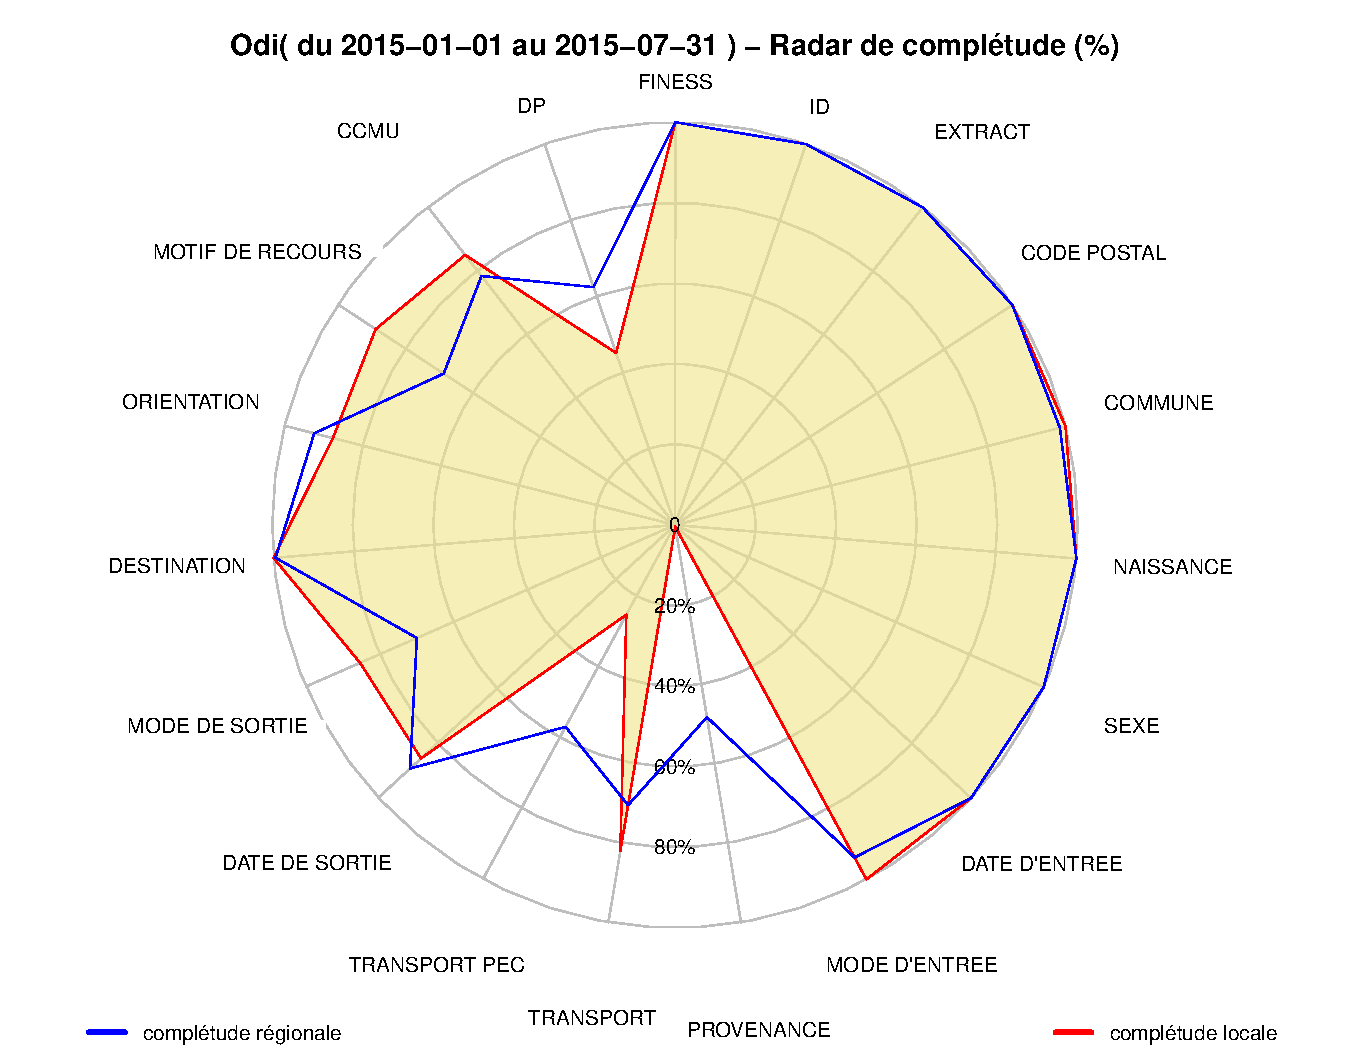
\includegraphics{completude_files/figure-latex/finess-14.pdf}

\begin{verbatim}
## Score local: 82.88  sur 100
\end{verbatim}

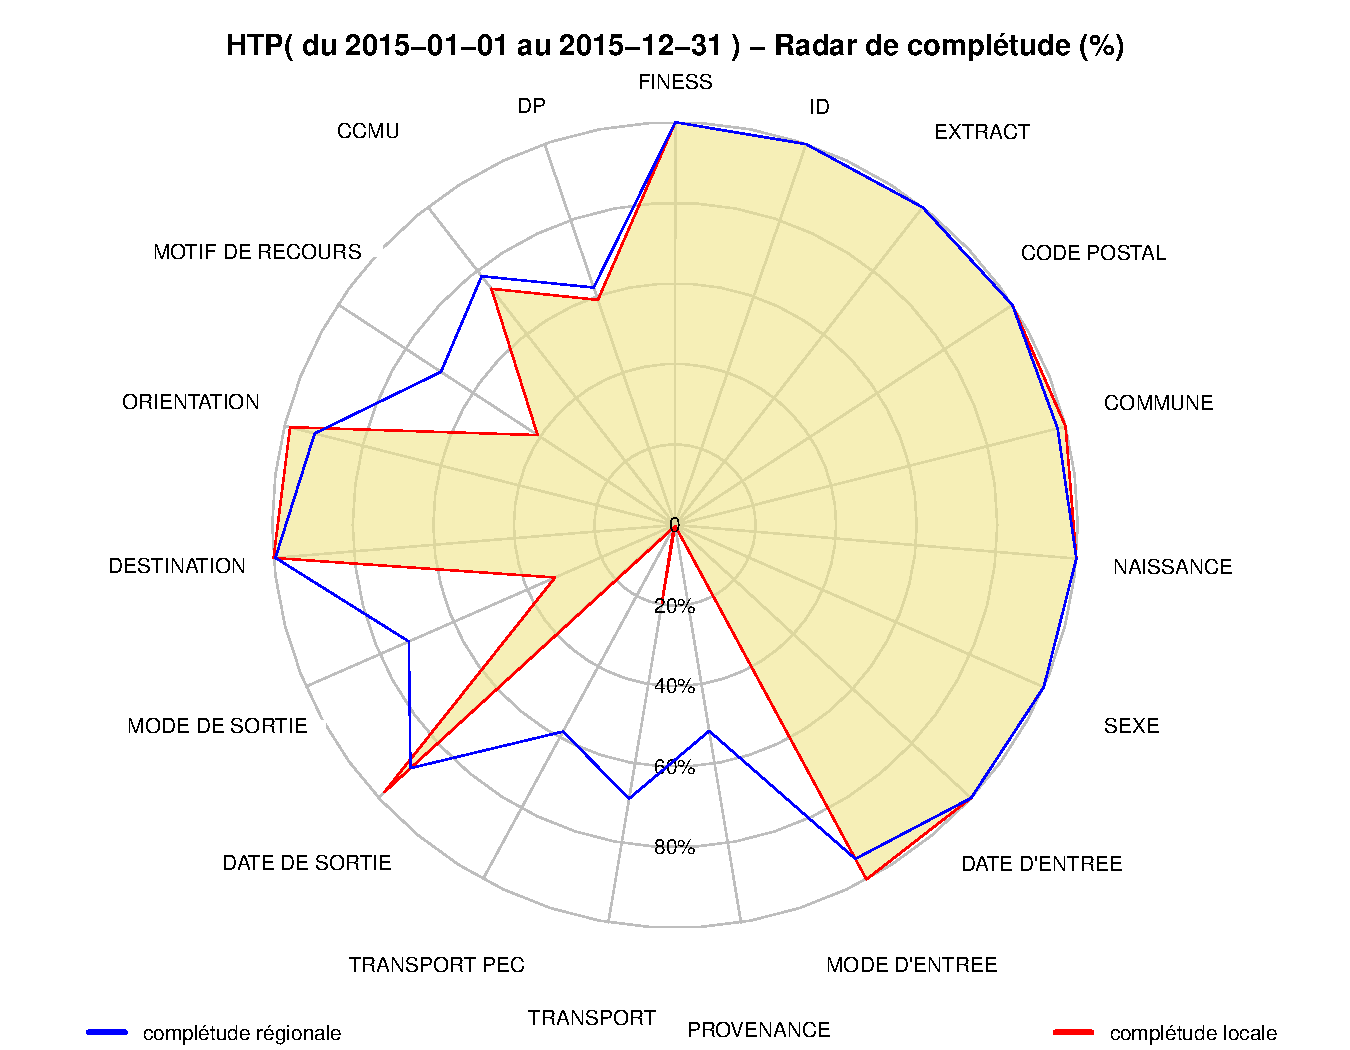
\includegraphics{completude_files/figure-latex/finess-15.pdf}

\begin{verbatim}
## Score local: 64  sur 100
\end{verbatim}

\subsection{Motif de passage}\label{motif-de-passage}

\end{document}
